%!TEX root = ../username.tex
\chapter{R-CNN Variation} \label{chap:rcnn_variation}

Since the interested domain for this paper is the object detection and instance segmentation task, we will analyze the Mask R-CNN. Mask R-CNN is a popular algorithm that tries to solve both object detection and instance segmentation problem in the Computer Vision field. However, Mask R-CNN is the improved version of Faster R-CNN and Fast R-CNN, which is based on the R-CNN algorithm. Therefore, to fully understand Mask R-CNN, we will start with understanding the building block of R-CNN, which is designed for object detection tasks.

\section{R-CNN}

R-CNN, also known as regional-based convolutional neural networks, is an object detection algorithm. The algorithm was developed by a group of researchers at UC Berkeley in 2015. Since its development, the R-CNN model has revolutionized the field of computer vision. The model was designed to detect up to 80 different types of objects in images and provide large-scale object recognition capabilities. Additionally, before the existence of RCNN, most algorithms in object recognition task used support vector machine (SVM) with blockwise orientation histograms like Histogram of Oriented Gradients (HOG) \cite{svm_hog} or Scale-Invariant Feature Transform (SIFT) \cite{svm_sift}. SVM dominated the space until 2012. In 2012, a CNN algorithm showed an astounding image classification accuracy on ImageNet Large Scale Visual Recognition Challenge (ILSVRC). Since then, more studies have been created into developing and improving algorithms utilizing CNN. The R-CNN model is our first attempt to build an object detection model that extracts features using a pre-trained CNN.

\begin{figure}[!ht]
    \centering
    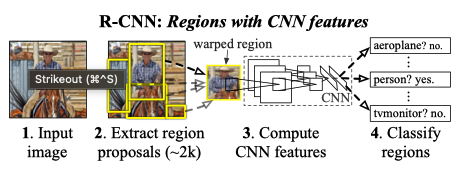
\includegraphics[width=4.5in]{figures/rcnn_archiet.png}
    \caption{R-CNN overall architecture \cite{Girshick_R_CNN_2013}} \label{fig:rcnn_archiet}
\end{figure}

In a board picture, the R-CNN model is composed of three modules [Fig. \ref{fig:rcnn_archiet}]. The first module's purpose is to generate regions of interest (RoI), i.e., regions that possibly contain an object. The second module utilizes a CNN to extract out feature vector from each proposed region. The third module then performs classification for each region using a pre-trained SVM algorithm on the feature vectors provided by the second module. As we can see R-CNN algorithm tries to find the location of each object, extract the object features, and classify these features. Next, we will dive deeper into each module of R-CNN.

\subsection{The First Module: Region Proposal}
In the first module, the algorithm used in this step must be able to propose some region of interest (RoI). A region of interest is a smaller part of the original image that could contain an object.

Given this problem, one might consider the bruce-force method by examining every small rectangle area of the original image as a potential region of interest in a systematic way. This method is the main concept behind the sliding-window technique, a type of exhaustive search algorithm used in the region proposal task. The sliding window technique involves running a window of a predefined size across the image, such that each subsection of the image is considered as a potential region proposal. Like the CNN kernel, the windows' size, stride, and padding are all customizable and can be adjusted to suit different types of images. In addition, multiple scales can also be incorporated into the sliding window technique, which allows for more robust performance in scenarios where objects may appear at different sizes within the same image. Since the sliding window technique examines every location within the image by considering every pixel as part of some RoI, it will not miss any potential object location. However, considering every location in the image as an RoI is unnecessary due to objects most likely not appearing everywhere in the image. Furthermore, classifying every sub-image at different sizes will require tremendous computational power. Therefore, even though it allows our model to detect all possible locations, the sliding window technique should not be used in autonomous cars' vision because it is computationally expensive.

In recent years, many studies have shown interest in improving the efficiency of the region proposal algorithm. One notable algorithm that gives the same strength as the sliding window technique is selective search. The selective search was designed to combine the strength of both exhaustive search and segmentation \cite{selective_search_2013}. The strength that selective search inherits from sliding windows is the ability to find all the possible locations that can be a potential region of interest. Additionally, selective search utilizes the underlying image structure to cluster pixels into different regions, taken from the strength of the segmentation technique. Selective search also aims to complete three goals. These three goals are to capture all scales, diversification, and fast to compute. Capture all scale is the idea that the algorithm must be able to detect objects of different sizes in the image. Next, diversification requirements refer to a method of grouping regions. The algorithm must be able to combine regions containing part of an object into one region. Additionally, for instance, like a person inside a car or a person in front of a car, the algorithm must be able to separate the region for the car and the region for the person under diversification requirement. Lastly, fast computing requires the algorithm not to demand heavy computational power.

As for selective search overall behavior, it can be thought of as two steps. The first step is to perform \textbf{bottom-up segmentation} -- described in Efficient Graph-Based Image Segmentation by Felzenszwalb and Huttenlocher \cite{felzenszwalb_huttenlocher_2004} -- to generate initial sub-segmentation. The second step is to combine similar sub-segmentation recursive using a similarity score between subsegments. The similarity score is a combination of four similarity grouping criteria. These four criteria are color similarity, texture similarity, size similarity, and fill similarity \cite{selective_search_2013}. The reason that color and texture similarity between regions is needed is that the same object most likely will have the same texture or shade of color. In the original paper, the color and texture similarity criteria score can be described by an equation only based on a fixed number of values taken from the histogram of each color channel. Thus, these two similarity scores require minimal to no computational power to compute. Similarly, two regions that have the majority of the area overlap with each other are most likely described the same object. Therefore, the use of a fill similarity score allows the algorithm to merge regions that mostly overlap and keep regions that are not overlapping separate from each other. The fill similarity score can be calculated using the following equation: 
%
\begin{equation*}
    S_{fill}(r_i, r_j) = 1-\frac{size(BB_{ij})-size(r_i)-size(r_j)}{size(image)}
\end{equation*}
%
where $r_i, r_j$ are two considering RoI, and $BB_{ij}$ is the bounding box around $i$ and $j$. Lastly, the similarity in size between the two regions takes into consideration to make sure that the algorithm identifies all locations for different objects at different scales. The size similarity score can be calculated using the following equation: 
%
\begin{equation*}
    S_{size}(r_i, r_j) = 1-\frac{size(r_i)+size(r_j)}{size(image)}
\end{equation*}
%
where $r_i, r_j$ are two considering RoI. As we can see, the similarity score computation is fast and take into account the diversification of the image data set. With these two steps, the selective search can quickly classify foreground and background, then downsample the number of potential RoI that existed in foreground segmentation. Therefore, utilizing selective search allow the model to reduce the number of falsified RoI compared to sliding window and requires lower computational power.

In the original paper of R-CNN, in the first module -- region proposal -- utilize selective search algorithm \cite{Girshick_R_CNN_2013}. However, as mentioned before, the R-CNN model can be thought of as three separate modules; thus, one can experiment with R-CNN with different region proposal techniques.

\subsection{The Second Module: Feature Extraction With CNN}
On completion of the first module of R-CNN, which generates all regions of interest within an image, these RoIs are passed to the AlexNet architect for feature extraction \cite{Girshick_R_CNN_2013}. AlexNet, a CNN architect, was proposed by Alex Krizhevsky at the University of Toronto in 2012 with the guidance of Ilya Sutskever and Geoffrey E. Hinton \cite{AlexNet_2017}. AlexNet was trained using ImageNet, which at the time was the most extensive picture data collection. As AlexNet required its input to have a fixed resolution with the same width and height, the photos in ImageNet were resized to $256 \times 256$ pixels. Prior to publication, AlexNet competed in ILSVRC-2010 and obtained top-one error rates of 37.5\%. In other words, 37.5\% of the time, the model assigns the highest score to the correct label. In the same competition, AlexNet also achieves top-5 error rates of 17.0\%, i.e., the correct label in the top 5 predicts 17\% of the time.

\begin{figure}[!ht]
    \centering
    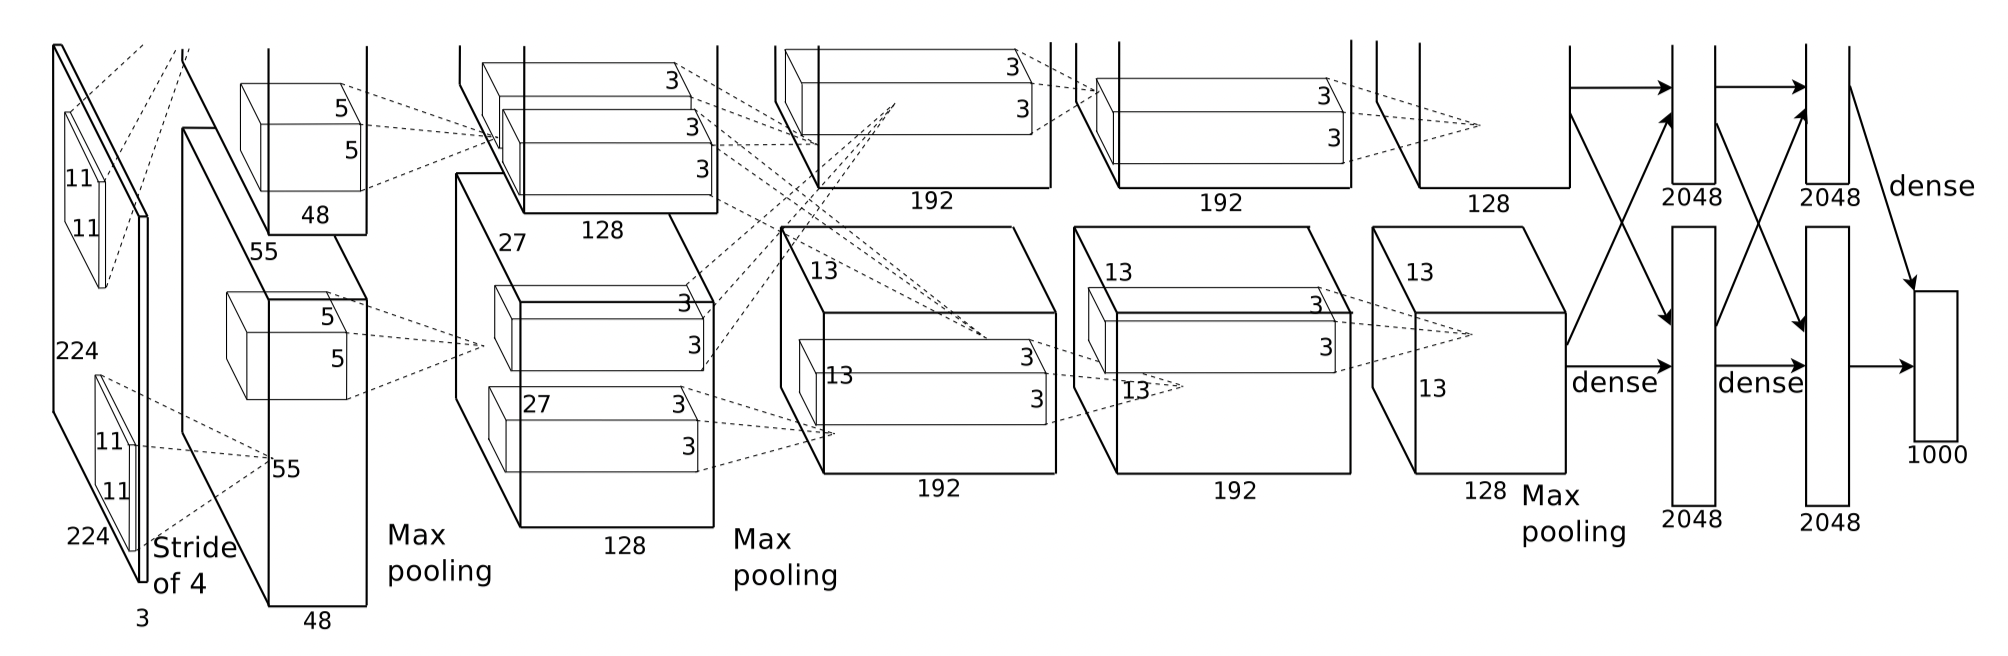
\includegraphics[width=6in]{figures/alex_net.png}
    \caption{AlexNet's overall architecture \cite{AlexNet_2017}} \label{fig:alex_net_architecture}
\end{figure}

AlexNet is regarded as one of CNN's most significant innovations. AlexNet, with 60 million parameters and 650,000 neurons as of 2012, is one of the largest neural networks ever suggested. The architecture of AlexNet consists of eight learned layers. Five convolutional layers are followed by three layers that are fully connected. Due to hardware limitations at the time, it was not possible to fit a massive network like AlexNet on a single GPU. For this reason, the model's architecture is distributed across two separate GPUs, and training must pass via both GPUs. Due to this limitation, for each layer in the network, the model has half of the neurons for that layer on each GPU and only requires particular layers to perform GPU communication. For example, in the overall architecture of AlexNet presented in Figure \ref{fig:alex_net_architecture}, we note that neurons of the first layer only connect to neurons of the second layer on the same GPU. On the contrary, we notice that all neurons of the second layer are fully connected with neurons in the third layer. The notion of spreading neurons across multiple GPUs is known as the parallelization scheme. The parallelization scheme is a topic that remains outside the scope of this paper, and GPU memory size is no longer a significant problem due to the current advancement of technology. Therefore, understanding the parallelization scheme is likely to be optional for the analysis of a CNN model.

In addition to being one of the largest networks and employing a parallelization strategy, AlexNet was among the first neural networks to employ ReLUs. The ReLUs activation function was employed instead of the more common $Tanh$ and $Sigmoid$ functions at the time because AlexNet was designed to reduce learning time. Using ReLUs, the model has a faster learning rate, which, according to the author, would vastly increase the performance of large models with a large data set. In addition, AlexNet implements local response normalization (LRN) to assist ReLUs in generalization. The non-trainable LRN layer is utilized following the first and second network layers. Following the first, second, and fifth layers, AlexNet employs a max-pooling layer with a size of 3 and a stride of two 2. The author notes that having an overlapping pooling layer — i.e., size 3 > stride 2 — decreases overfitting in general \cite{AlexNet_2017}.

AlexNet employs data augmentation and dropout techniques to address the issue of overfitting when training an extensive network with a large data set. For data augmentation, AlexNet randomly selects images into batches and resizes them to a resolution of $224 \times 224$. It then generates a copy with horizontal reflection image transformation and a copy with modified intensity for the three RGB channels. The CPU generates these transformed images while the GPU trains on the previous batch, allowing the data augmentation process to be done without incurring any additional performance costs. In addition to data augmentation, AlexNet also uses the dropout technique. If the output of any hidden neurons is less than or equal to 0.5, the network sets its output to 0. This technique reduces the computation required because neurons with 0 need not be considered in the rest of the forward pass or updated during backpropagation. This method also permits neurons in the network to be independent of one another, as no neurons are guaranteed to persist with each training sample.

R-CNN model utilizes the AlexNet architect implemented on the Caffe framework. R-CNN model passes each generated RoI as a separate image to AlexNet for feature extraction. Since the RoI role is to find each object location in the image, thus AlexNet can assume each RoI only have exactly one object. AlexNet also requires image input of fixed resolution $224 \times 224$; thus, R-CNN transform to the required size by warping all pixels in a bounding box of $227 \times 227$.

\subsection{The Third Module: Classification With Pre-trained SVM}

\begin{figure}[!ht]
    \centering
    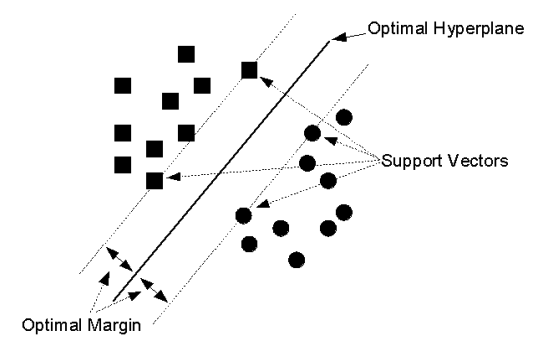
\includegraphics[height=2in]{figures/2d_svm.png}
    \caption{2D linear SVM visualization \cite{2d_svm_Tzotsos}} \label{fig:2d_svm_viz}
\end{figure}

After the second module, R-CNN is able to obtain multiple features for each RoI. Each RoI with extracted features then be given to each trained linear SVM classifier in each class for evaluation. Since each class has its own SVM classifier, thus the SVM only needs to distinguish between objects belonging to the class and objects that are not belonging to the class. Linear SVM classifier can be thought of as trying to draw a $N-1$ dimension separator in the $N$-dimension space where $N$ is the number of features of a specific class. The separator in SVM must be linear, and it tries to separate objects in the class and objects outside of the class. The best-fit separator has the highest margin between any point in the class and any point outside of the class. An example of 2-dimensional linear SVM is visualized by figure \ref{fig:2d_svm_viz} where the circle represents the object in this class, and the square is the object outside the class. Given that the class-specific SVM know what features the class possesses. The separation between objects in and out of the class can be done with little computation power, as we already have the extracted features. Each class SVM is then given the RoI a score representing the likelihood that the object in RoI belongs to this class. Therefore, for each RoI, the class with the highest SVM score is assigned to be the class for the object.

\subsection{R-CNN Result and Drawback}
On the PASCAL VOC dataset 2012, by combining these three modules, R-CNN achieved 53.3\% in \textbf{mean Average Precision (mAP)}. R-CNN also achieves the mAP of 31,4\% and ranks first on the ILSVRC2013 dataset in terms of accuracy \cite{Girshick_R_CNN_2013}. Despite achieving an incredible breakthrough in using Convolutional Networks and having a high object detection accuracy, R-CNN's performance is marred by a number of disadvantages. These issues include multi-stage training, high runtime and space complexity, reliance on non-learnable algorithms, and slowness \cite{fast_rcnn_og}. 

As described by the architecture of R-CNN, the network is divided into three modules and runs sequentially. The network attempts to feed the input of one module with the module's output coming before it. In other words, the first module must completely process the image before the second module is running. Therefore, the network's modules must wait on one another and be trained individually, thus creating the multi-stage training problem. Secondly, since the first module generates 2000 proposed RoIs before the second module can start running, the networks must cache these proposed RoIs on the disk. Similarly, the generated feature for each RoI must be stored on the disk before processing by SVM. The need to write and read multiple time for each RoI cause a high order of runtime and space complexity. The runtime and space complexity is even higher when we consider overlapping RoIs; the network recalculates features and classification for the overlapping portion of overlapping RoIs. Thirdly, the selective search algorithm used in the first module is a non-learnable algorithm. Therefore, the algorithm runtime and accuracy would not improve through training the network. Additionally, through the error analysis, the author notices the mass amount of localization inaccuracy. Thus, for each proposed region, after being scored by the SVMs, the region is piped to a class-specific bounding-box regressor to generate a new bounding box. Finding the bounding box within the region of interest allows the model to improve localization accuracy but exacerbates the model runtime performance as it generates the bounding box at least twice for each object in the image. Lastly, with a processing speed of 47s per image, the R-CNN model is slow and thus has limited real-world application.

\section{Fast R-CNN} \label{sec:fast_rcnn}

The author of R-CNN later implemented Fast R-CNN to reduce the runtime and space complexity while improving detection accuracy. Fast R-CNN is implemented in Python and C++. Like the R-CNN model, Fast R-CNN can be used along with any convolutional neural network. In the proposal Fast R-CNN model, the author utilized VGG16, a one of the deepest CNN in 2015, as the backbone CNN for the model. Comparing the performance of Fast R-CNN with VGG16 versus R-CNN with VGG16 on the PASCAL VOC 2012 dataset, while having the same setup, the experiment showed that Fast R-CNN is 9 times faster at train-time and 213 times faster at test-time while achieving a higher mAP score \cite{fast_rcnn_og}. In the next section, we will mention the keynote of VGG16 architecture, follow by the discussion of Fast R-CNN model and its design decisions that lead to a higher mAP.

\begin{figure}[!ht]
    \centering
    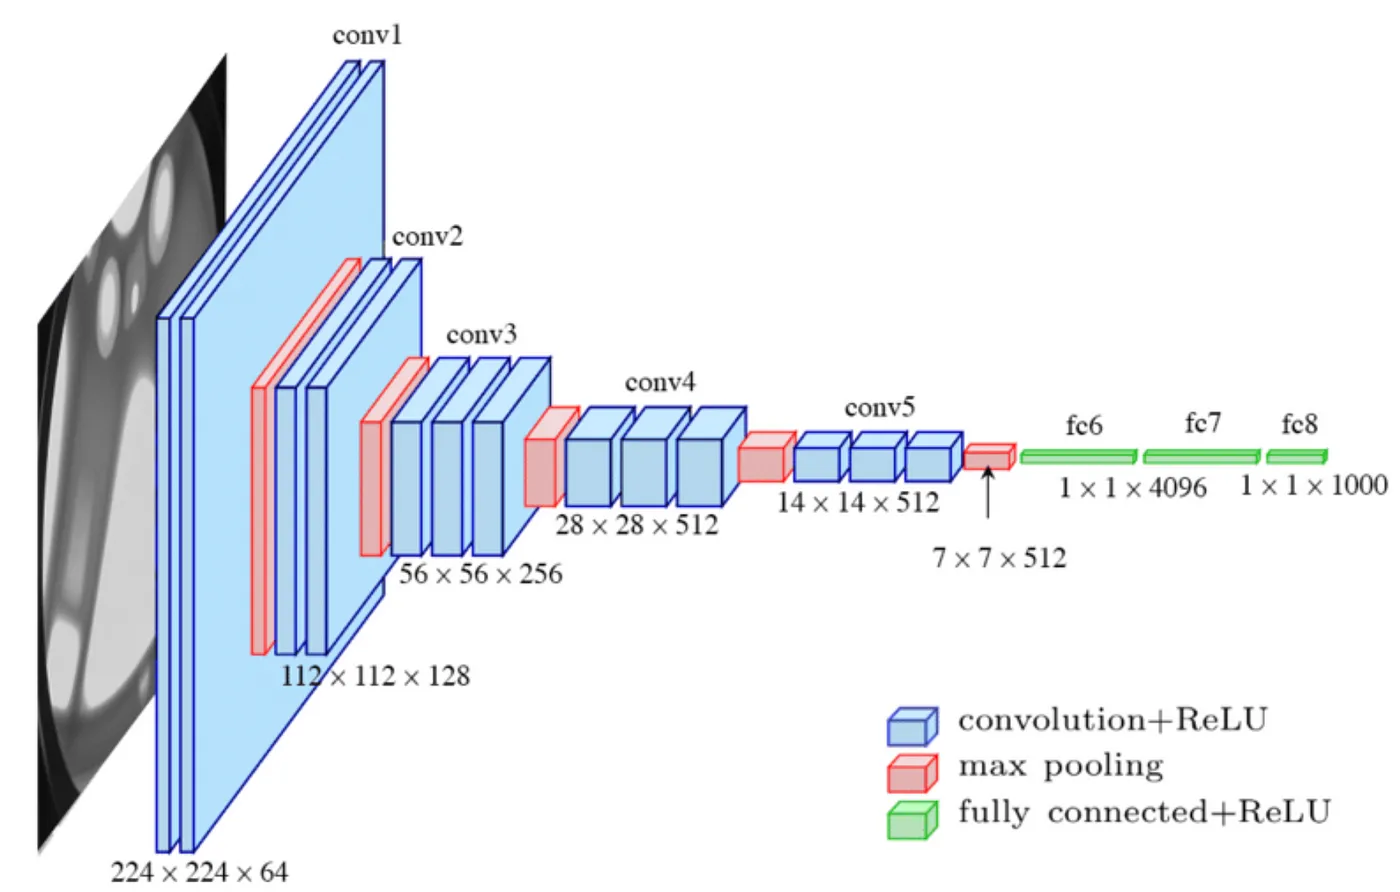
\includegraphics[width=4in]{figures/vgg16_architect.png}
    \caption{VGG16 architecture \cite{vgg16_architect_2014}}
    \label{fig:vgg16_archite}
\end{figure}

The VGG16 is a CNN model developed by the Visual Geometry Group (VGG) at the University of Oxford in 2014 \cite{vgg16_2014}. The VGG16 architecture is notably deeper than AlexNet, comprising 16 learnable layers -- 13 convolutional layers and 3 fully connected layers -- and 5 non-trainable max-pooling layers [Fig. \ref{fig:vgg16_archite}]. VGG16 takes an RGB $224 \times 224$ image as input and generates a $7 \times 7$ feature map, downsampled by a factor of 32 from the input image resolution \cite{deconv_rcnn_2018}. A set of fully connected layers is then processed this feature map to produce the predicted classification label for the image. Unlike AlexNet, which uses a combination of $3 \times 3$ and $5 \times 5$ filters, VGG16 uses only $3 \times 3$ filters throughout the network with smaller strides and padding. By employing a strategy like utilizing a pair of stacked $3 \times 3$ layers in place of a single $5 \times 5$ layer, VGG16's design enabled it to demonstrate that elevating the depth of a network to 16 layers can yield substantial improvements for existing CNNs. Fast R-CNN adapts any CNN model for object detection by performing three changes. The first change is replacing the last pooling layer with an RoI pooling layer (named RoIPool). For VGG16, an RoI will be used in place of the $7 \times 7 \times 512$ max-pool layer in Fast R-CNN. The second change is replacing the last fully connected layer with two sibling layers, i.e., replacing the fc8 layer for VGG16. Lastly, Fast R-CNN will adjust the input layer of the CNN model to accept images of any size and proposed RoIs for that particular image as input. We will discuss these changes in more detail later in this section.

\begin{figure}[!ht]
    \centering
    \subfloat[][Overall architecture \cite{fast_rcnn_og}]{ 
        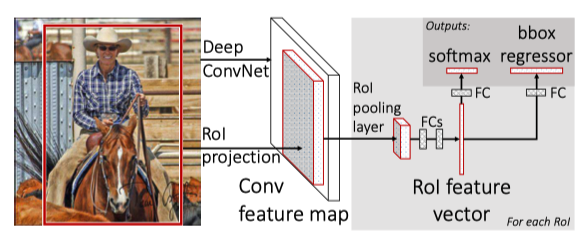
\includegraphics[width=3in]{figures/fast_rcnn_archiet.png} \label{fig:fast_rcnn_archite} 
    }

    \subfloat[][Network flow \cite{rcnn_vari_flow_chart}]{ 
        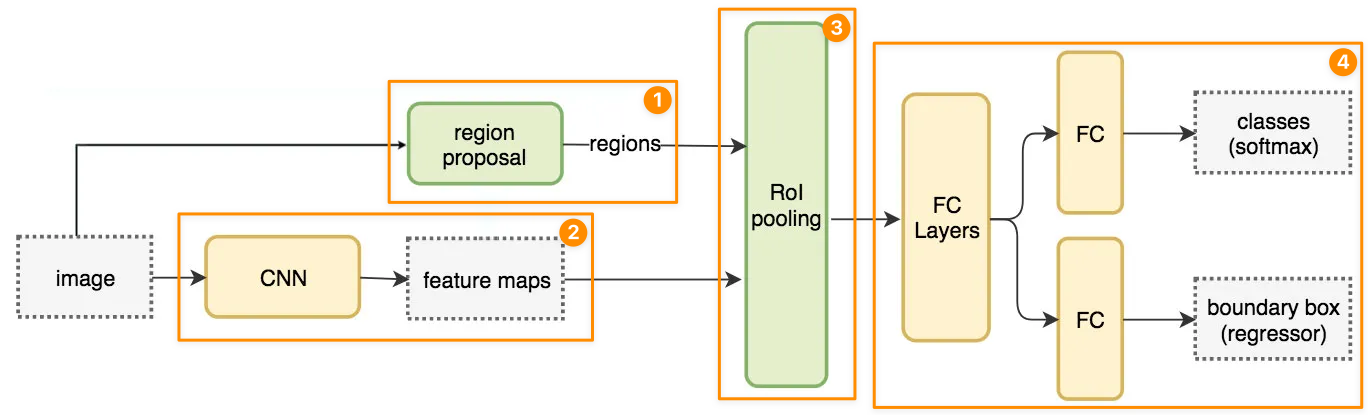
\includegraphics[width=5.5in]{figures/fast_rcnn_flowc.png} \label{fig:fast_rcnn_flowc} 
    }
    \caption{Fast R-CNN overall architecture and network flow} \label{fig:fast_rcnn_archite_flowc}
\end{figure}

The overall architecture of Fast R-CNN can be thought of as four stages [Fig. \ref{fig:fast_rcnn_archite_flowc}]. The network takes an image and a set of RoI as inputs. Comparing Fast R-CNN with R-CNN, which takes an image as an input and then generates RoIs with selective search, the type of input data between the two models is not equivalent. Thus we assume Fast R-CNN takes an image as input and performs the selective search algorithm as the first stage of the model. In the second stage, Fast R-CNN generates a feature map for the entire image by running the input image through a CNN. The CNN used for Fast R-CNN performance measurement in the original paper is VGG16. In the third stage, the model use RoIPool layer to extracts the feature grid corresponding to the proposed RoI from the image feature map generated in stage two for each proposed RoI. The RoIPool layer is also used for downsampling the RoI feature grid of any size to a pre-defined fixed-length feature vector. In the fourth stage, each RoI feature vector is processed by multiple fully connected layers and then branched into the two sibling output layers -- softmax classification and bounding box regression. The model's learning with two output branches is possible with the use of multi-task loss.

\begin{figure}[!ht]
    \centering
    \subfloat[][R-CNN architecture with stages]{ 
        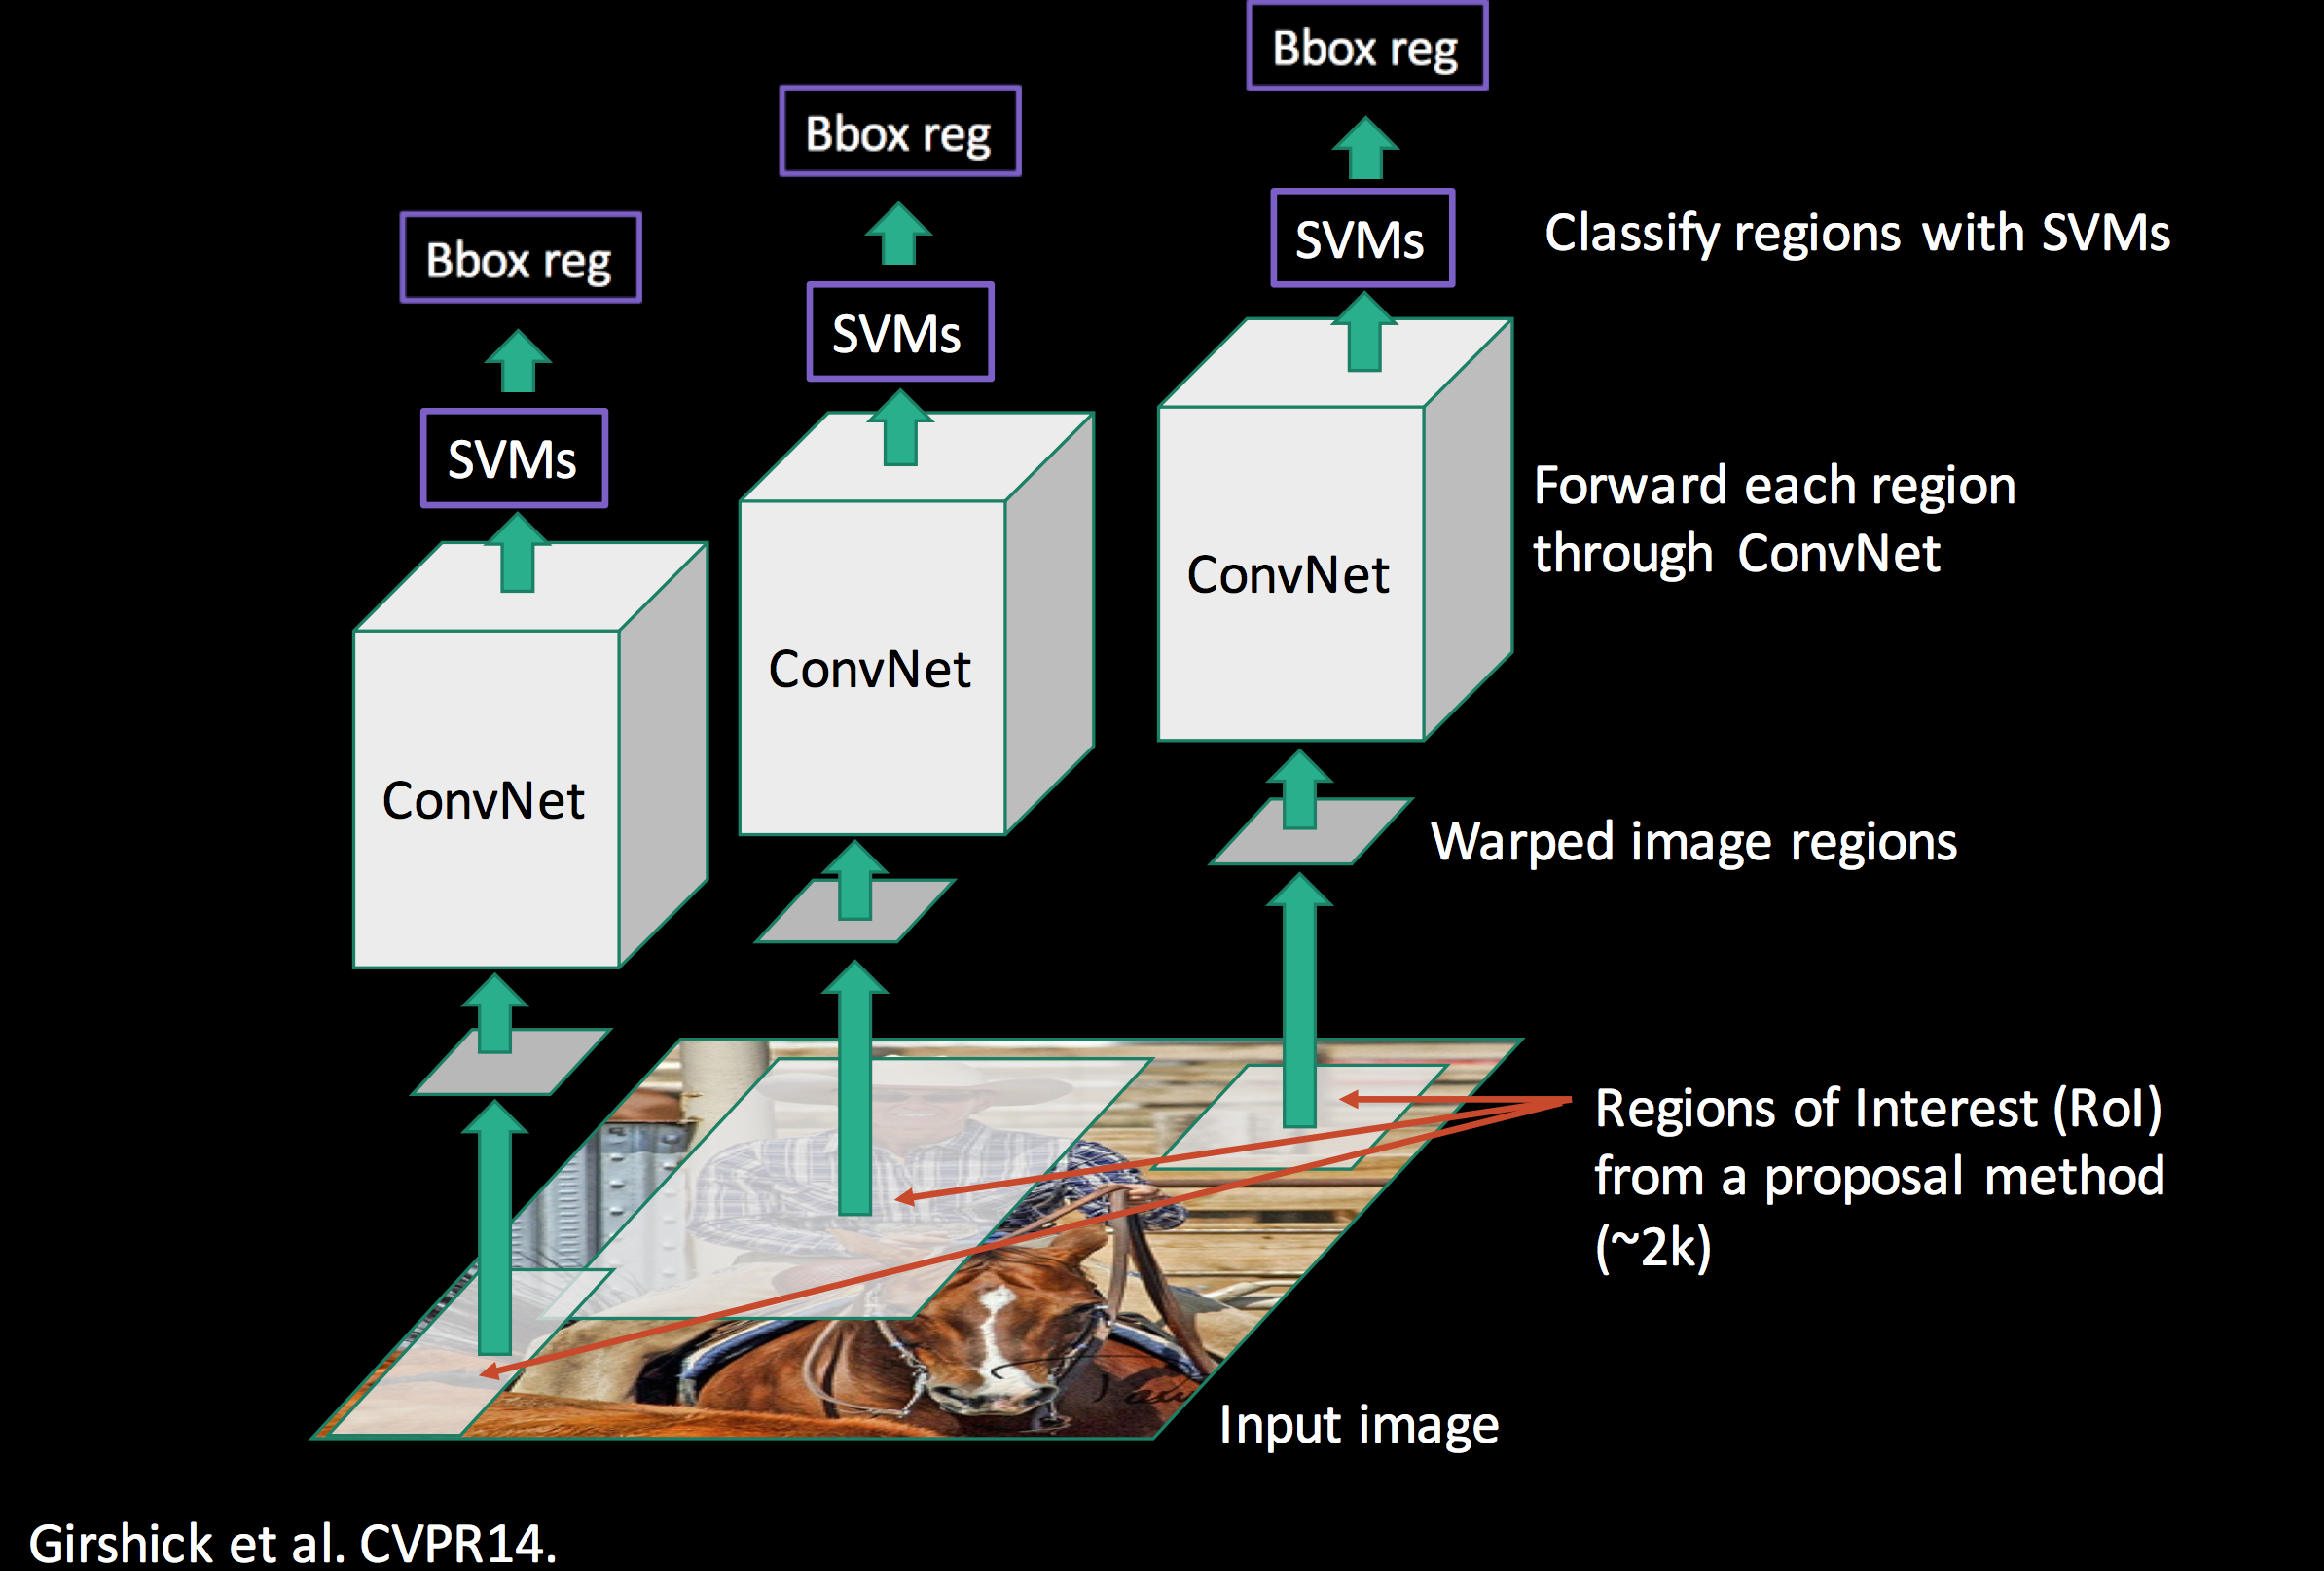
\includegraphics[height=2in]{figures/rcnn_custom_draw.png} \label{fig:rcnn_custom_draw} 
    }
    \subfloat[][Fast R-CNN architecture with stages]{ 
        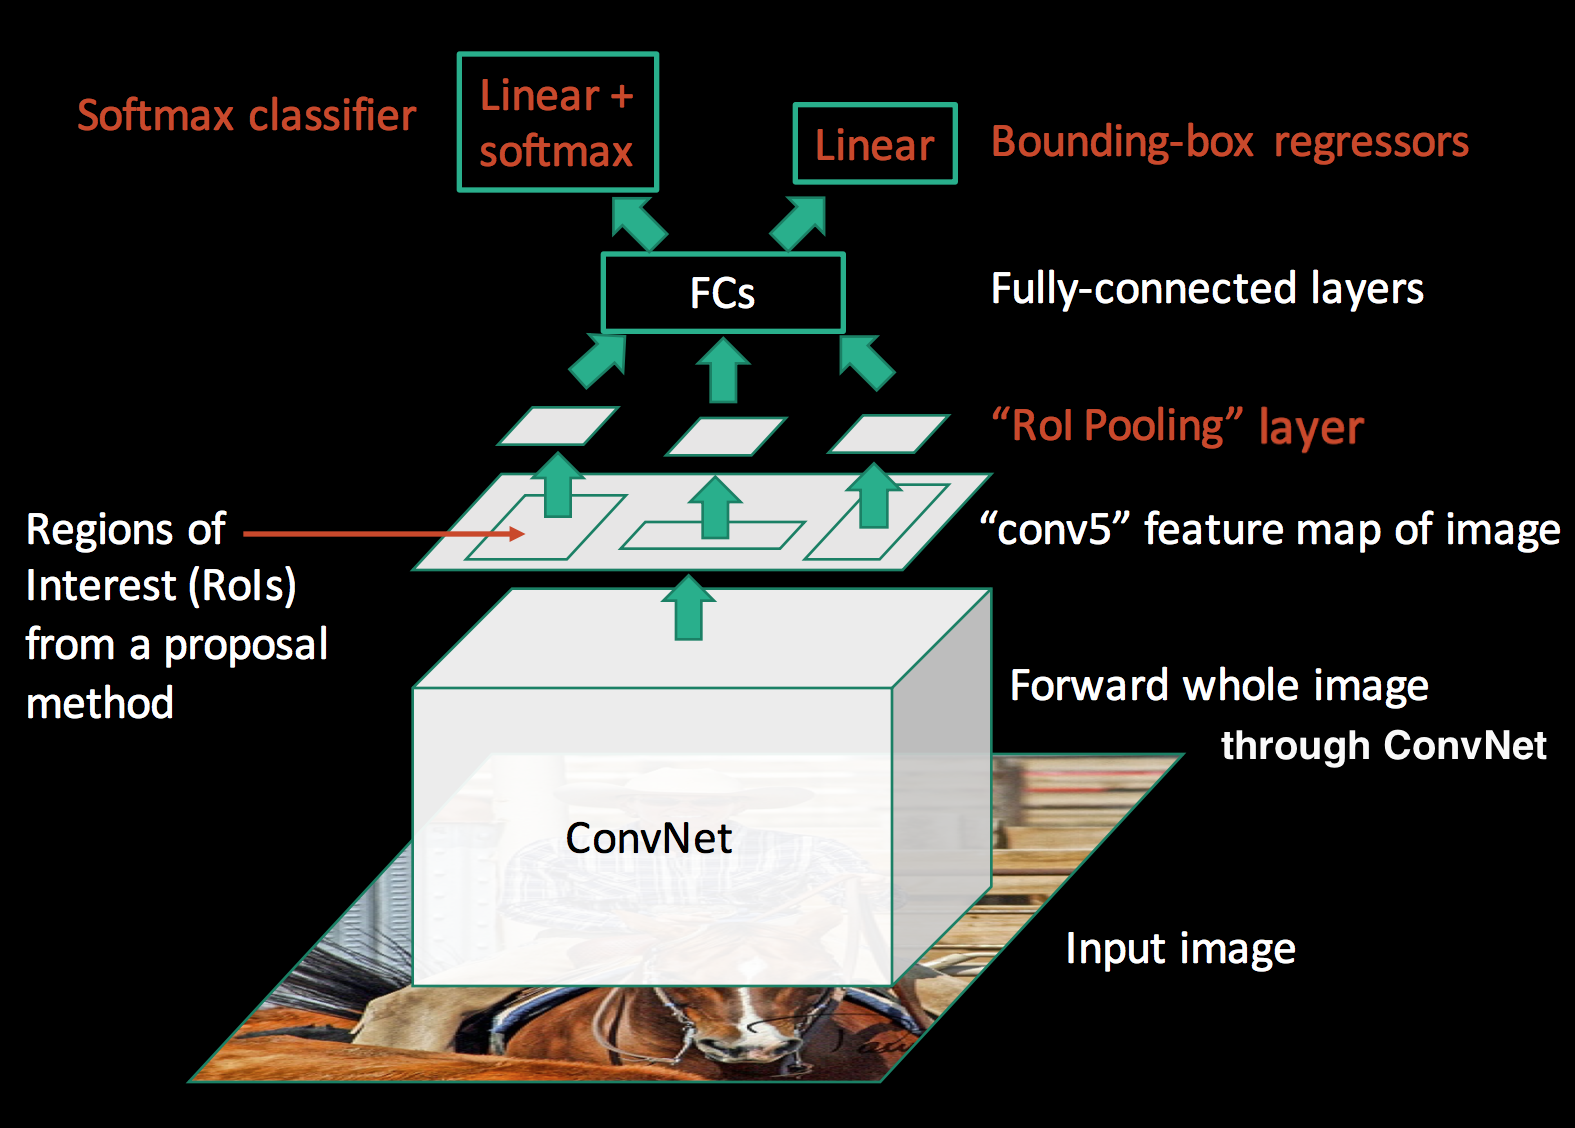
\includegraphics[height=2in]{figures/fast_rcnn_custom_draw.png} \label{fig:fast_rcnn_custom_draw} 
    }
    \caption{R-CNN vs. Fast R-CNN architecture comparision \cite{rcnn_vs_faster_custom_fig}} \label{fig:rcnn_vs_fast}
\end{figure}

Comparing the architecture of R-CNN and Fast R-CNN, there are three main differences between the two models [Fig. \ref{fig:rcnn_vs_fast}]. The first difference is that Fast R-CNN generates the feature map for the entire input image instead of each RoI individually. This means Fast R-CNN only applies CNN to image one and shares the feature maps across RoIs. Fast R-CNN behavior holds several advantages compared to treating RoIs individually, like in the R-CNN model. These advantages are reducing the use of disk storage, reducing redundancy operation performed on overlapping RoI, and sharing computation power and memory used between RoIs in the same image, thus improving the performance at test-time \cite{fast_rcnn_og}. Sharing the feature map and memory data between RoIs also allows the model to be trained faster. The author reported that training Fast R-CNN by examining multiple RoIs in an image allows the model to convert roughly 64 times faster compared to when trained with RoIs from different images. 

The second difference is the inclusion of the RoI pooling layer (named RoIPool). This layer is responsible for extracting RoI feature grids of varying sizes and downsampling them to a fixed pre-defined size. To extract the RoI feature grid for any input RoI, the RoIPool layer first maps the top left corner point of the input RoI box, which is defined on the input image, to a corresponding pixel in the feature map. Then, the width and height of the input RoI are reduced by the same factor that the feature map is downsampled from the original image. As we will perform a max-pooling operation on the pixels' value, the size of the original projected RoI must be rounded down to the nearest integer because we cannot take a partitioned pixel. After projecting the top left corner and rounding the scaled-down RoI size from the input layer onto the feature map, we have the offset rounded projected RoI. The RoI feature grid is then formed by every feature map pixel that lies inside this offset rounded projected RoI. Since objects in the input image can have different sizes and aspect ratios, thus the projected RoI feature grid can also vary in size. However, the input of a fully connected layer must be of the same pre-defined size, which is why the input's size independent downsampling operation is necessary. The RoIPool layer achieves size-independent downsampling by dividing the RoI feature grid into a pre-defined $W \times H$ grid of RoI bin (or RoI bin), where $W \times H$ is the required dimension for the following fully connected layer input. In other words, the layer divides the $w \times h$ RoI feature grid into RoI bins of equal size, each with an approximate size of $\frac{w}{W} \times \frac{h}{H}$. Here, $\frac{w}{W}$ and $\frac{h}{H}$ represent the number of pixels along the width and height of the RoI bin, respectively, and are rounded down to the nearest integer. In contrast to the traditional pooling layer described in Sec. \ref{subsec:pooling_layer}, which used a sliding technique dependent on the input size, the division into a grid of equal RoI bins enables the RoIPool layer to have a fixed output grid size regardless of the size of the layer's input RoI. The RoIPool layer then applies max-pooling to the pixel values in each RoI bin, thereby effectively reducing the size of any projected RoI to a pre-defined $W \times H$ size.

The third difference is going from multi-stage training in R-CNN to single-stage multi-task training in Fast R-CNN. In R-CNN, the model must be completely trained with class-specific SVM before being trained with class-specific bounding box regressor, and these tasks also are performed in the same sequence in the test time. On the contrary, Faster R-CNN has the softmax classifier and bounding box regressor as sibling output layers. Fast R-CNN model generates a multi-task loss $L$ for each RoI and uses the loss $L$ as a metric to jointly train both the softmax classifier and bounding box regressor branches. The multi-task loss $L$ is generated from the difference between the truth label, truth box, and predicted label, predicted box perspectively. The author suggested that employing a multi-task learning scheme would improve performance, as the network's shared components must be general and precise enough to produce correct results for both classifier and bounding box regressor branches \cite{fast_rcnn_og}. The author also reports that Fast R-CNN with multi-task learning consistently achieved higher mAP scores than stage-wise training across different CNN implementations.

These changes in architecture allow the Fast R-CNN model to achieve a processing runtime of 0.3 seconds per image, excluding the time needed for object proposal \cite{fast_rcnn_og}. However, when factoring in the runtime for object proposal, such as the Selective Search algorithm, Fast R-CNN is almost 7.67 times slower, taking 2.3 seconds per image \cite{selective_search_2013}. Additionally, the RoIPool layer in Fast R-CNN causes the model to undergo quantization. Quantization is the process of reducing the precision of an input from a large set of possible values to a smaller set of discrete values. Recall that the RoIPool layer initially projects the input RoI box to the appropriate location, rounded down to the nearest pixel in the feature map. The layer then subdivides the projected RoI, expressing the size of each RoI bin in the projected RoI in terms of pixels. In other words, the RoIPool layer quantizes these sizes and coordinates from the continuous non-negative real number set to the discrete natural number set. While quantization enables the layer to perform a valid max-pooling operation on pixel values, it also introduces a loss of precision and information in our model. The loss in precision is caused by the projected RoI deviating slightly from its actual coordinate. The loss in pixel data is due to the RoI RoI feature grid cannot always be divided perfectly without remainder.

\begin{figure}[!ht]
    \centering
    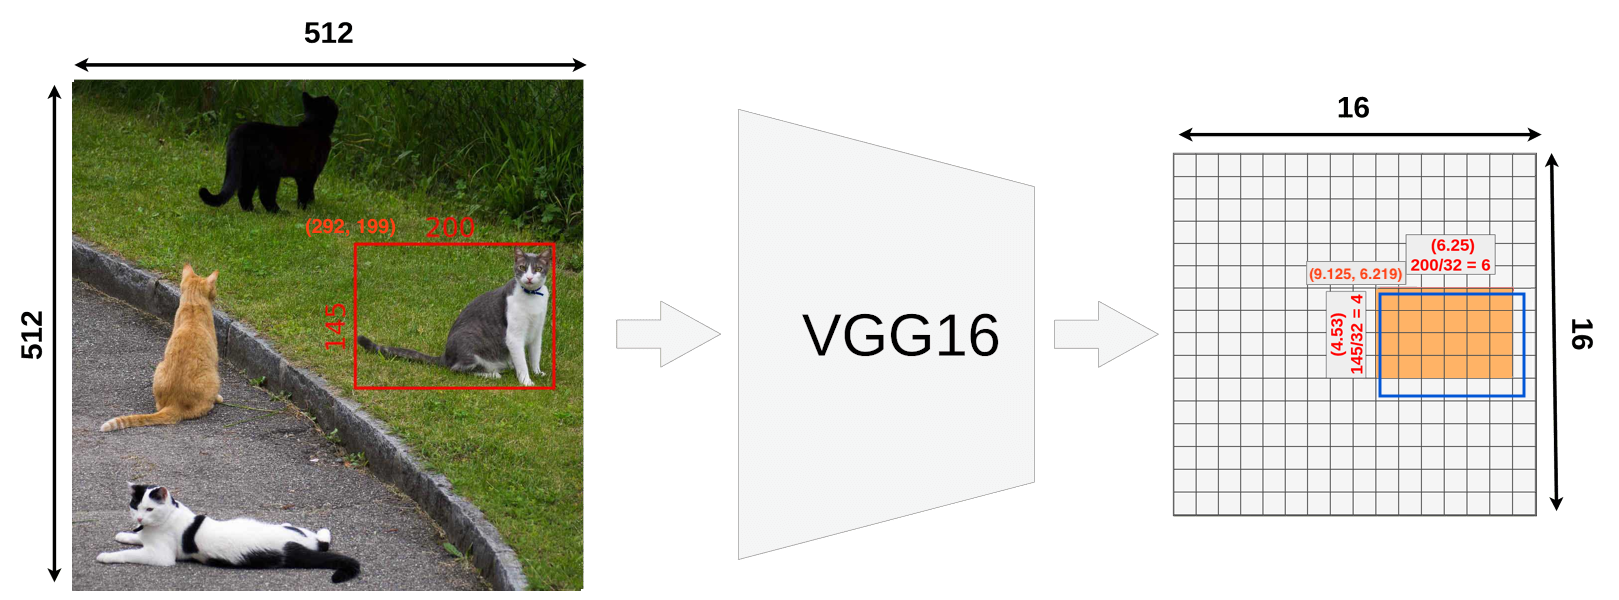
\includegraphics[width=6in]{figures/roi_projection_ex.png}
    \caption{RoI projection to feature map \cite{roi_pooling_problem}}
    \label{fig:roi_projection_ex}
\end{figure}

As an example, assume that we are processing an input image of $512 \times 512$ with VGG16, and the first fully connected layer expects $3 \times 3$ as input [Fig. \ref{fig:roi_projection_ex}]. Consider the input RoI with the top left corner coordinate of $(292, 199)$ and the size of $145 \times 200$. As mentioned earlier, VGG16 has a scale-down factor of $32$ from the input image to the feature map space. With this information, we can compute the corresponding coordinate and size of the input RoI in the feature map as follows:
\begin{align}
    &\text{Feature map RoI corner coordinate: } &\left( \floor{\frac{292}{32}}, \floor{\frac{199}{32}} \right) \ \ &= \ \ \left( \floor{9.125}, \floor{6.21875} \right) \ \ &= \ \ (9, 6) \\
    &\text{Feature map RoI size: } &\floor{\frac{200}{32}} \times \floor{\frac{145}{32}} \ \ &= \ \ \floor{6.25} \times \floor{4.53125} \ \ &= \ \ 6 \times 4
\end{align}
When projecting to the feature map space, Fast R-CNN offsets and resizes the original projected RoI (shown as the blue rectangle in Fig. \ref{fig:roi_projection_ex}) to align perfectly with $n$ feature map pixels (shown as the orange area in Fig. \ref{fig:roi_projection_ex}), where $n$ is the number of feature map pixels that can fit entirely within the original projected RoI. As shown in Fig. \ref{fig:roi_projection_ex}, we lose some pixels data (white part inside the blue rectange), and have additional noise datas (orage part outside the blue rectange). Consider the quantization of the conner's vertical position at 6.21875 to 6 in feature map space. When we factor in the scaling of 32 times, this means our projected RoI is shifted by $(6.21875 - 6) \times 32 = 7$ pixels vertically compared to the input RoI in the original image space. Similarly, the projected RoI is offset by 4 pixels horizontally, and the quantization process results in a loss of $(0.25 + 0.53125) \times 32 = 25$ pixels during projection.

\begin{figure}[!ht]
    \centering
    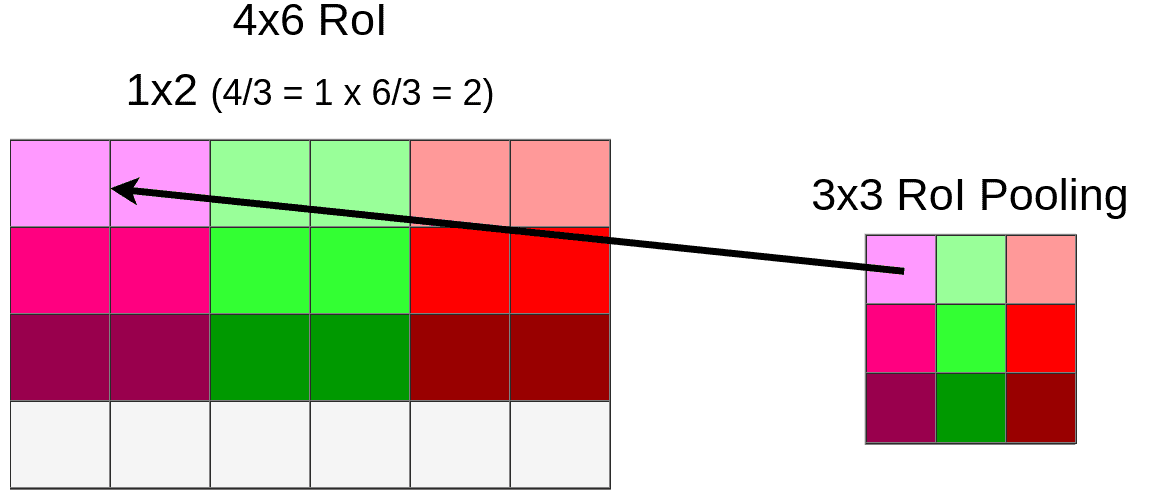
\includegraphics[width=4in]{figures/roi_pool_ex.png}
    \caption{The RoI feature grid is divided into RoI bins, as shown on the left. Performing max-pooling on each RoI bin results in a $3 \times 3$ output matrix, as shown on the right. Each cell in the input image represents a feature map pixel, and each RoI bin contains 2 pixels and has a unique color. Each cell in the output $3 \times 3$ matrix represents the highest feature map pixel out of all pixels in each corresponding RoI bin. The white cells on the left do not belong to any RoI bin and are not used in the RoI pooling process.\cite{roi_pooling_problem}}
    \label{fig:roi_pool_ex}
\end{figure}

After projecting and quantizing the input RoI, we obtain an RoI feature grid. In our example, this grid has dimensions of $6 \times 4$ and is located at position (9, 6). However, the next layer in our network requires inputs of size $3 \times 3$. To accommodate this, we divide the RoI feature grid into a grid of RoI bins, each with a size of $\frac{6}{3} \times \frac{4}{3} \approx 2 \times 1.3333$. Since these sizes are expressed in terms of pixel counts, we must quantize them to the nearest integer values, resulting in RoI bins of size $2 \times 1$. As shown in Fig. \ref{fig:roi_pool_ex}, this quantization results in the loss of information for the bottom row of pixels in the RoI feature grid, corresponding to a loss of $6 \times 32 = 192$ pixels in the input image space. In addition, the pooling operation can also cause small offsets in the position of the RoI bins, leading to further loss of information. Combined every loss happen in the RoIPool layer, the model has loss $192+25=217$ pixels. In addition, the RoI used for classification is offset by 7 pixels vertically and 4 pixels horizontally. While the loss of 217 pixels due to quantization and pooling may seem small compared to 29,000 pixels in the input RoI of size $200 \times 145$, thereby, can be overlooked in the object detection task. However, as the goal of our study lies in the instance segmentation task, where the model outputs a mask containing every pixel belonging to the object, every pixel counts. Nonetheless, these loss in information and offset is for one input RoI. Due to the fact that object identification tasks typically detect multiple objects per image, the loss of information and offset caused by quantization may compromise the quality of the model. 

To address the quantization issue in the RoIPool layer, RoIAlign was proposed as a method for achieving size-independent downsampling without quantization. The RoIAlign is utilized with Mask R-CNN, an instance segmentation model that will be discussed in greater detail in Sec. \ref{sec:mask_rcnn}. Since Mask R-CNN is built on top of Faster R-CNN, which is also the subsequent significant improvement over the Fast R-CNN model, we will discuss the Faster R-CNN model in the following section. Faster R-CNN proposes the addition of the region proposal network (RPN) to resolve the bottleneck in object detection performance caused by object proposal runtime \cite{faster_rcnn_2015}. Instead of attempting to reduce the runtime of the object proposal algorithm, RPN's primary objective is to share computation with the object classification module, thereby allowing the object detection model to generate object proposals at no additional cost. We will further discuss the region proposal network (RPN) used in conjunction with Fast R-CNN to create Faster R-CNN in section \ref{sec:faster_rcnn}.

\section{Faster R-CNN}

\section{Mask R-CNN} \label{sec:mask_rcnn}